%%%%%%%%%%%%%%%%%%%%%%%%%%%
\chapter {Introduction}
\label{INTRO}
%%%%%%%%%%%%%%%%%%%%%%%%%%%

  A distributed system is a group of computational entities that collaborate with each other in order to achieve one or more tasks. Telecommunication systems are an example of distributed systems.  In order to accomplish certain goals, these computational entities follow a set of behavioural rules referred to as a distributed protocol. The distributed system environment is usually presented in a graph composed of nodes and edges. The nodes represent the computational entities while the edges represent the communication links between entities.  

One interesting aspect of distributed systems is distributed mobile computing which uses mobile agents. Mobile agents are computational entities with the ability to move from one node to a neighbouring node. The mobile agent model provides an excellent computing paradigm for distributed applications and has thus been extensively studied. These mobile agents can be used to perform many tasks including network management and maintenance (see \cite{kimetal}).

In this thesis we will use the mobile agent model in order to solve our problem. In this chapter we will provide the motivation behind this thesis, present our contribution and provide an overview of the organization of the thesis. 



\section{Motivation} 

Security is one of the main concerns when using distributed systems.  Many security threats have been discussed in the literature, such as {\em black hole} and {\em contamination}. The presence of those threats in any network can cause serious malfunctions. The mobile agent model has been proposed as one of the solutions to cleaning a network that has been affected by these threats.  

In this thesis we investigated a fairly new threat called the \bv that was initially introduced by Cai et al. in \cite{caietal18}.  A \bv  is a faulty node that is able to destroy any visiting mobile agent without leaving a trace. Moreover, the \bv clones itself onto other \bvs with the same capabilities and each copy moves to a neighbouring node and stays inactive until triggered by a visiting agent. This behaviour leads to serious repercussions such as  network disconnectivity. A \bv can only be cleared if it arrives at a node that is already occupied by an agent.


The nature of the \bv  is quite destructive since its location  is unknown a priori and it has the ability to move to neighbouring nodes. We require a solution that searches the system until the \bv is located and triggered and then sends mobile agents to guard the neighbouring nodes of the \bvs that have just been created by the original one(\cite{caietal18}).  Besides effectiveness, one important consideration when searching for a solution to this problem is cost. The main elements that should be taken into consideration when attempting to solve the black virus decontamination problem are:  the size of the team of mobile agents, the overall number of {\it black viruses} and the total number of moves required for the mobility of the agents.




%---------------------------------
\section{Our Contribution} 


We first conduct a thorough survey of the literature for two problems that are closely related to our topic:  {\it   black hole search} and {\it decontamination}. We then review \cite{caietal18}, the only paper that addresses the existence of a \bv in a network.

In \cite{caietal18}, the authors  address the problem of black virus decontamination in different regular graphs. One interesting regular topology that commonly models distributed systems and that has not been the subject of study is the  {\em Chordal Ring} (also called a {\em Circular Graph}). A chordal ring is an augmented ring that is known for its fault-tolerance \cite{manetal5,baretal9} and symmetric properties \cite{baretal8}. It is for these same reasons that some of its variants are also commonly used as  peer-to-peer structures  \cite{floetal17, floetal30, stoetal10}. Chordal rings have been studied for many different reasons including routing  \cite{manetal6,caietal7}, dynamos  \cite{floetal31} and catastrophic fault patterns \cite{nayetal2,nayetal3}.



% TO BE PUT IN THE CORRECT FORMAT

%Paola Flocchini, Miao Jun Huang, Flaminia L. Luccio: Decontaminating Chordal Rings and Tori Using Mobile Agents. Int. J. Found. Comput. Sci. 18(3): 547-563 (2007)

%Bernard Mans, Nicola Santoro: Optimal Fault-Tolerant Leader Election in Chordal Rings. FTCS 1994: 392-401

%Bernard Mans: On the Interval Routing of Chordal Rings. ISPAN 1999: 16-21

%Jin-yi Cai, George Havas, Bernard Mans, Ajay Nerurkar, Jean-Pierre Seifert, Igor Shparlinski: On Routing in Circulant Graphs. COCOON 1999: 360-369


%Lali Barri�re: Symmetry properties of chordal rings of degree 3. Discrete Applied Mathematics 129(2-3): 211-232 (2003)

%Lali Barri�re, Josep F�brega, Ester Sim�, Marisa Zaragoz�: Fault-tolerant routings in chordal ring networks. Networks 36(3): 180-190 (2000)

%Paola Flocchini, Amiya Nayak, Ming Xie: Enhancing peer-to-peer systems through redundancy. IEEE Journal on Selected Areas in Communications 25(1): 15-24 (2007)

%Paola Flocchini, Fr�d�ric Geurts, Nicola Santoro: Optimal irreversible dynamos in chordal rings. Discrete Applied Mathematics 113(1): 23-42 (2001)

%Ion Stoica, Robert Morris, David Liben-Nowell, David R. Karger, M. Frans Kaashoek, Frank Dabek, Hari Balakrishnan: Chord: a scalable peer-to-peer lookup protocol for internet applications. IEEE/ACM Trans. Netw. 11(1): 17-32 (2003)

%%% ADD TO THE BIBLIO THE WORK ON CATASTROPHIC FAULT PATTERNS.


In this thesis we investigated the {\it  Black Virus Disinfection} problem in chordal rings using the mobile agent model in a synchronous environment. Our main focus was on the initial existence of one \bv and how to minimize its disruptive effect on the entire topology.  Our primary goal was to minimize the complexity of the problem in terms of number of agents, number of moves and spread of the virus.
 


We investigated the problem in undirected chordal rings labelled with a chordal sense of direction and proposed     monotone  disinfection strategies. A monotone strategy means that once a node is explored it stays clean and never gets re-infected.

The team of agents is lead by a coordinator whose task is to direct the decontamination activities. The leader can create new agents and assign specific tasks.
All of our solutions work in two phases: {\em Exploring and Shadowing} and {\em Surrounding and Eliminating}. 

In the first phase the team searches the the topology using safe exploration techniques until the \bv is located. This phase is terminated by the activation of the original \bv and the creation of more \bvs at unguarded nodes that have now been discovered by the leader. This phase is common to all chordal ring types studied in this thesis.


The second phase involves surrounding the newly-created \bvs by deploying agents to their neighbouring nodes. After all the neighbours are guarded, the leader activates the \bvs    by sending agents to their specific locations. As expected, the \bvs move to the neighbouring nodes, which are now guarded, and get destroyed. 

Deploying agents is the most critical part of this phase. The deployment can be done in various settings. In this thesis, we discuss two variations: {\em local} and {\em non-local}. 



The non-local strategy guarantees optimal routing because  the leader, which  has  full topological knowledge,  manages the whole process:  it sends the surrounding agents to their destinations through the shortest path and  the surrounding agents carry the whole path to their destinations
  ({\em Move-Optimal Deployment}). For all the topologies considered in the thesis, we calculated an upper bound on the optimal move complexity, where the bound is tight for particular chord structures.
     
  
With local strategies,  the surrounding agents plan the path to their destinations according to the local information they have and deploy to their target   by making local choices at each intermediate node without having to carry the full routing path. Whenever possible, we propose alternative local strategies, all based on greedy choices.
More precisely, in this thesis we will have the following: 
\begin{enumerate}
\item  In the case of the double loop chordal ring, we will describe  three deployment strategies: simple greedy, smart greedy and move-optimal. For the move-optimal deployment,  we will also indicate the shortest paths to reach all of the targets for any chord structure. The greedy strategies are not optimal, however, they are local and efficient.
\item In the case of the triple loop chordal ring, the local greedy strategies will not work due to the complex chord structure. As a result we will focus only on the non-local approach. The  leader has full topological knowledge and is able to calculate  the shortest path to the targets. We are able, however,  to calculate their exact length  only for particular triple loops with simpler chord structures, while in the general case, we find only  upper bounds to the optimal length.
\item In the case of consecutive-chord chordal rings, we describe a local strategy (the one-direction greedy) since it provides the shortest path to the target.  
\item Finally, for general chordal rings with any chord structure, we describe a local strategy that is  not optimal but efficient and gives upper bounds to the optimal length. 
\end{enumerate}










%---------------------------------

\section{Thesis Organization} 

In this section, we will present the organization of the thesis. After this chapter we review literature on topics related to our problem. We begin by reviewing some papers that address the black hole search problem in different settings, variations and topologies. We then review some papers concerning the decontamination problem, sometimes referred to as intruder capture, in different settings and variations. Finally, we review the only paper that investigates black virus disinfection in several topologies.

In chapter  3  we introduce the problem in question and provide definitions and terminology regarding black virus disinfection. We also present our assumptions and topology (the chordal ring) and describe the high level ideas that serve as the basis for all of our solutions.

In chapter 4 we go through our solution for double loop chordal rings where every node has just one chord in addition to the ring link. 
We describe in detail the two phases and  their complexities. For the second phase, we  introduce  three deployment strategies: {\em Move-optimal}, {\em Simple greedy} and {\em Smart greedy}. For the move-optimal deployment strategy, we present the solution for two cases: shortly-chorded double loops (where the non-ring chord is small compared to the size of the ring) and the general double-loop.  Our bound on the move-complexity is tight for shortly chorded double loops.

In chapter 5 we address the problem in  triple loop chordal rings. 
We describe in detail the two phases and  their complexities. For the second phase, we  describe only the move-optimal strategy since the greedy approach does not work for this type of chord structure. For simplicity, we only consider  the shortly-chorded triple loops in the calculation of the upper bound on the number of moves. We also show that the  bound is tight in  two special extreme cases.

In chapter 6 we address the problem in chordal rings with consecutive chords.   For  the second phase, we describe only a local greedy strategy (One-direction greedy) because it also provides an optimal-move solution for this particular chordal ring.

In chapter 7 we discuss the problem in  arbitrary chordal ring structures. 
The surrounding solution that we propose is very general and works with any chord structure, however, it is not  optimal. We provide upper bounds to the path lengths. 


In chapter 8 we conclude our thesis by summarizing all the results and discussing some open problems related to the \bv disinfection topic.







\begin{figure}[H]
  \centering  
  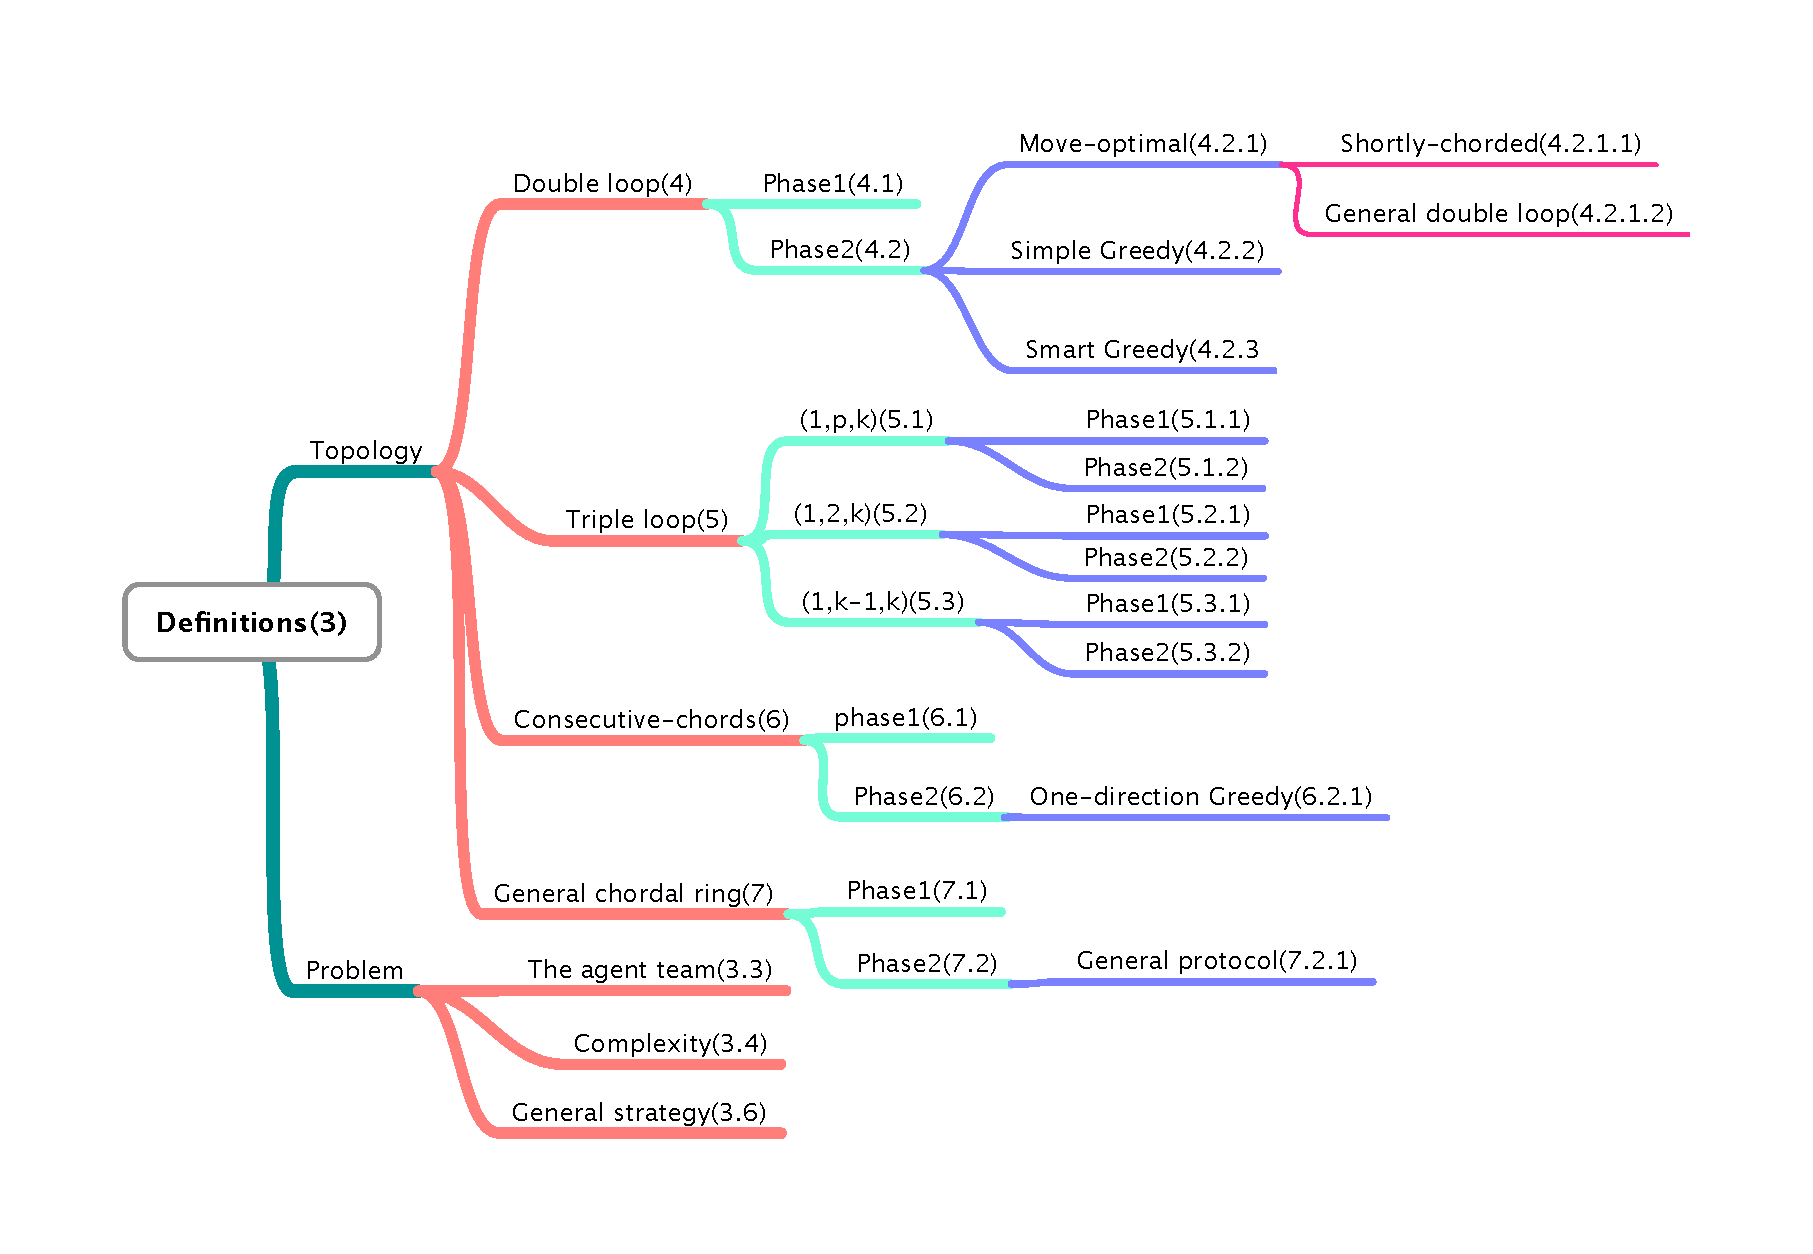
\includegraphics[width=1\textwidth]{figures/map2.pdf}
  \caption{A map showing the organization of the thesis}
\end{figure}


